\section{Expériences empiriques}
\label{sec:emp}

Cette section sera l'occasion de valider numériquement les garanties présentées à la
Section \ref{sec:bound} quant aux erreurs de généralisation et de sous optimalité
inhérentes à l'algorithme d'investissement présenté dans ce mémoire.

Il va sans dire que le cadre théorique général qui a été développé jusqu'à maintenant
présente plusieurs paramètres (dimensionalité du problème, loi de marché, fonction
d'utilité, noyau employé, etc.); tous les décrire représenterait une tâche titanesque,
aussi certains choix devront être faits pour restreindre la quantité de paramètres
étudiés; la Section \ref{emp:metho} énumérera le choix fait pour chacun de ces paramètres.

Par la suite, les Sections \ref{emp:nvar}, \ref{emp:pvar} et \ref{emp:npvar} étudieront la
qualité des garanties de généralisation et de sous optimalité dans un contexte où,
respectivement, la taille de l'échantillonage augmente ($n$ variable, $p$ constant), la
taille de l'échantillonage est fixe mais la dimensionalité du problème augmente ($n$
constant, $p$ variable) et enfin, la taille de l'échantillonage et de la dimensionalité
augmentent toutes les deux, mais à des rythmes différents.



\subsection{Méthodologie}
\label{emp:metho}

\paragraph{Noyau}

Le noyau employé dans nos expériences sera linéaire, \ie\ $q(x) = q^Tx$. En particulier,
c'est avec un tel noyau que la dépendance entre la dimensionalité du problème et les
erreurs de sous optimalité et de généralisation se caractérise le plus facilement (voir
Section \ref{b:dim}).

\paragraph{Fonctions d'utilité}

Chaque expérience sera conditionnée par une fonction d'utilité exponentielle Lipschitz
$\LEU_\mu$ définie algébriquement par
\begin{equation}
  \LEU_\mu(r) = 
  \begin{cases}
    r & r<0\\
    \mu(1-e^{-r/\mu}) & r\geq 0
  \end{cases}.
\end{equation}
pour $\mu \geq 0$ (voir la Figure \ref{fig_leus}). Cette famille de fonctions d'utilités est
intéressante pour deux raisons: de telles fonctions ont toutes un coefficient Lipschitz
$\gamma = 1$ et leur paramètre $\mu\geq0$ permet de quantifier facilement l'aversion au risque
qu'elles convoient, $\mu = \infty$ correspondant à une attitude neutre au risque et
$\mu = 0$ correspondant à l'attitude extrêmement averse où aucune utilité n'est accordée aux
rendements supérieurs à zéro (semblable aux fonctions de perte \textit{hinge loss} en
classification).

La fonction d'utilité inverse $\LEU_\mu^{-1}:\Ut\to\R$, nécessaire pour exprimer en terme de
rendement équivalent les erreurs exprimées en util, est illustrée à la
Figure \ref{fig_leu_inv}. On peut vérifier algébriquement que
\begin{equation}
  \LEU_\mu^{-1}(r) =
  \begin{cases}
    r & r<0\\
    -\mu\log(1-r/\mu) & r\geq 0
  \end{cases}.
\end{equation}

Finalement, les bornes d'erreur de généralisation et de sous optimalité, lorsqu'elles sont
exprimées en équivalent certain, font intervenir l'inverse multiplicatif
$1/\partial_r u(r)$ du sous-gradient de la fonction d'utilité. Dans le cas d'une utilité
$\LEU_\mu$, cet inverse correspond simplement à l'inverse de la dérivée de $\LEU_\mu$ et est
donc donné par
\begin{equation}
  \left(\frac{d}{dr} LEU_\mu(r)\right)^{-1} = 
  \begin{cases}
    1 & r<0\\
    e^{r/\mu} & r\geq 0
  \end{cases}.
\end{equation}


\paragraph{Régularisation}

Sauf exception, le facteur de régularsation $\lambda = 1/2$ sera employé au cours de toutes les
expériences. 


\paragraph{Loi de marché}

La loi de marché $M$ sera construite en deux temps. D'abord, une loi de marché théorique
$\tilde M \in \Re^{\bar p+1 \times \bar p+1}$ sera construite selon la méthode présentée au
prochain paragraphe. Puis, un échantillon fini $M \sim \tilde M^{\num{5000}}$ de 5000 points
en sera tiré afin de former une loi de marché discrète $M$ à partir de laquelle toutes les
expériences seront réalisées. En quelque sorte, $M$ fournit alors une approximation à
$\tilde M$, mais permet de déterminer exactement des statistiques qui ne pourraient
autrement n'être qu'estimées, comme l'utilité hors échantillon $\EU(q)$ d'une politique
$q$, la décision optimale $q^\star$ ou l'utilité espérée optimale $\nEU^\star$ de la loi de
marché.

Pour construire la loi théorique $\tilde M$, chacune de ses lois marginales
$X_1,\ldots,X_{\bar p}$ et $R$ sera décrite par une variable aléatoire Rademacher (retournant
$\pm 1$ avec probabilité $1/2$).  La dépendance entre ces lois marginales sera modélisée
par une copule gaussienne dont la matrice de corrélation $\Sigma$ sera de la forme
\begin{equation}
  \Sigma =
  \kbordermatrix{
    &X_1 & \cdots & X_{\bar p} & R\\
    X_1& \ddots & & & \rotatebox{90}{\text{---}}\\
    \vdots  & & I_{\bar p\times \bar p} && \rho\\
    X_{\bar p}&&&\ddots &\rotatebox{90}{\text{---}}\\
    R & \text{---} & \rho & \text{---} &1},
\end{equation}
avec
\begin{equation}
  \rho = \left(\begin{matrix}\sqrt{\frac{1-\epsilon}{\bar p}} & \cdots & \sqrt{\frac{1-\epsilon}{\bar p}}\end{matrix}\right)
\end{equation}
sauf exception.

Le paramètre $\epsilon>0$ permet de quantifier l'idée que cette loi de marché n'admet pas
d'arbitrage puisque $R$ conserve alors une faible indépendance par rapport aux variables
de marché $X_j$. La Figure \ref{fig_copula} présente \num{1000} réalisations de cette loi
de marché $\tilde M$ lorsque $\bar p = 2$. Chaque point indique une réalisation de la loi
normale multivariée de matrice de corrélation $\Sigma$. Les lois marginales Rademacher de
$\tilde M$ font s'``effondrer'' ces valeurs à leur signe; les quatre histogrammes donnent
la fréquence d'un rendement positif ou négatif selon la valeur des deux variables de
marché.

Par ailleurs, pour ce cas particulier de loi de marché théorique, on peut établir que la
corrélation entre $X_j$ et $R$ correspond au \textit{tau de Kendall}, \ie\ $\Corr(X_j,R) =
\tfrac{2}{\pi}\arcsin\rho$. Voir \cite{remillard2013statistical} pour des précisions.

La valeur $\epsilon = 0.05$ sera employé au cours de toutes les expériences. De plus, on obtient
dans de telles conditions trivialement $\|X\| \leq \xi = \sqrt{p}$ et $\rmax = 1$.


\paragraph{Validation des garanties}

Les garanties énoncées à la dernière section s'appliquaient de façon probabiliste à
l'ensemble des réalisations hors échantillon. Les expériences suivantes mesureront, sauf
exception, le 95\ieme percentile d'erreur en employant $m=150$ échantillons d'erreur. Le
paramètre $\delta$ de confiance des deux bornes sera fixé à 95\%.

Plus précisément, $m$ échantillons $\S_n$ seront tirés indépendamment et identiquement de
$M^n$. Chacun de ces $m$ échantillons fournira une politique de décision
$\qh = \alg(\S_n)$ dont l'erreur de généralisation et de sous optimalité pourra alors être
calculée. Puis, de ces $m$ observations d'erreur, le 95\ieme percentile d'erreur pourra
finalement être calculé.

\paragraph{Progression de l'erreur}

Bien que les garanties sur l'erreur de généralisation et de sous optimalité donnent une
borne ``numérique'', elles suggèrent aussi une progression de l'erreur
$\bigO(p/\sqrt{n})$. On cherchera donc à vérifier cette ``suggestion'' en dévoilant
progressivement de nouveaux échantillons et/ou de nouvelles variables de marché afin de
vérifier l'évolution de l'erreur par rappport aux garanties théoriques.

Au début de chaque expérience, un ensemble d'entraînement formé de $\bar n$ réalisation de
$\bar p$ variables de marché seront tiré de $M$. Puis, on exposera progressivement à
l'algorithme $n$ des $\bar n$ points et $p$ des $\bar p$ variables de marché de cette
ensemble d'entraînement afin d'obtenir peu à peu une meilleure représentation de $M$. Le
tout sera répété $m$ fois (donc sur $m$ ensembles d'entraînement) afin de pouvoir mesurer
le 95\ieme percentile des deux types d'erreur.

Le premier ensemble d'expériences (Section \ref{emp:nvar}) conservera $p=2$ fixe et fera
varier $n$ de 2 à 110. À la Section \ref{emp:pvar}, ce sera la dimensionalité du problème
qui variera, donc avec $n$ fixe et $p$ variant de 1 à 50. Enfin, à la section
\ref{emp:npvar}, la situation sera un mélange des deux précédentes: plus en plus de points
provenant d'un même échantillon sont présentés à l'algorithme, leur dimension dévoilée
progressant en fonction de $n$.



\paragraph{Environnement de calcul}

L'identification numériques des politiques optimales $\qh$ se fera à partir de
l'implémentation CVXPY\cite{cvxpy} et du solveur ECOS\cite{ecos}. Les calculs numériques
se feront à partir de la librairie BLAS et de l'interface NUMPY.

\newpage



\begin{figure}[ht]
  \centering
  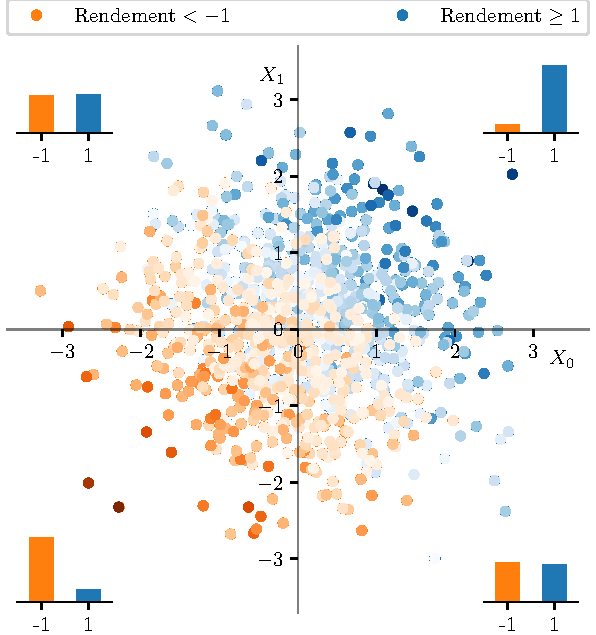
\includegraphics[width=\textwidth]{../experiments/fig/copula.pdf}
  \caption[Loi de marché]{Loi de marché théorique pour $\bar p = 2$. Les points bleus et
    orangés indiquent \num{1000} réalisations d'une loi normale multivariée avec matrice
    de corrélation $\Sigma$. Les lois marginales Rademacher de la loi de marché entraînent un
    ``effondrement'' des réalisations en $X_0$, $X_1$ et $R$ à leur signe. Les quatre
    histogrames présentent la distribution de $R$ par rapport à $X_0$ et $X_1$. On
    constate par ailleurs l'absence d'arbitrage d'une telle loi de marché.}
  \label{fig_copula}
\end{figure}


\begin{figure}[ht]
  \centering
  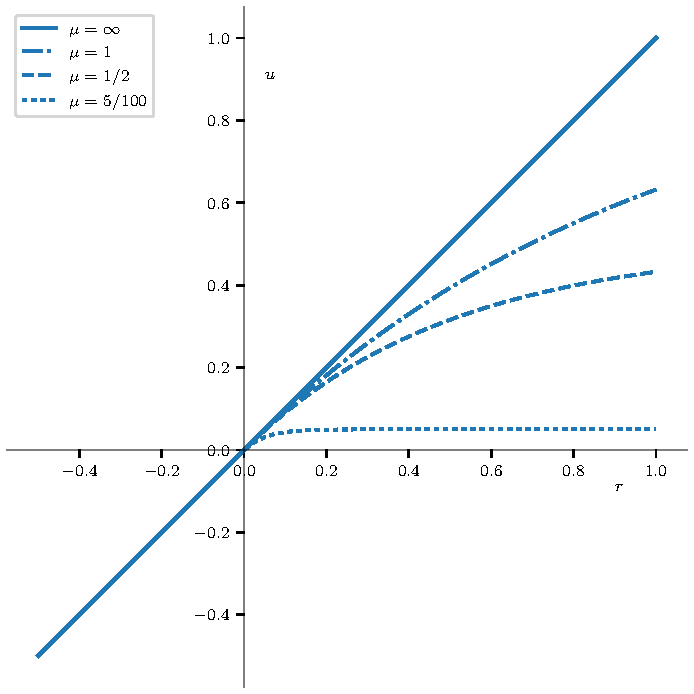
\includegraphics[width=\textwidth]{../experiments/fig/leus.pdf}
  \caption[Utilités LEU]{Comportement des fonctions d'utilité exponentielles Lipschitz
    $\LEU_\mu$ selon le paramètre $\mu$. L'abscisse est l'axe des rendements, alors que
    l'ordonnée est celui des \textit{utils}. Le paramètre $\mu$ de chacune des instances
    $\LEU_\mu$ permet de quantifier l'aversion au risque : un paramètre $\mu\to\infty$ indique une
    attitude neutre au risque, alors qu'à l'autre extrême, un paramètre $\mu\to0$ modélise une
    indifférence (utilité constante) aux rendement positifs. Sur la branche négative,
    l'utilité correspond à la fonction identité, sur la branche positive,
    $\LEU_\mu(r) = \mu(1-e^{-r/\mu})$.}
  \label{fig_leus}
\end{figure}

\begin{figure}[ht]
  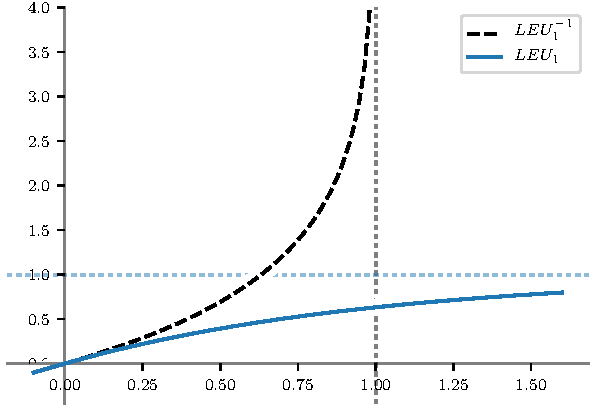
\includegraphics[width=\textwidth]{../experiments/fig/leu_inv.pdf}
  \caption{Utilité et utilité inverse. La fonction d'utilité permet de caractériser en
    \textit{utils} le rendement observé. L'\textit{util} est cependant une notion
    abstraite qu'on peut réexprimer en rendement à partir de la fonction utilité
    inverse. Une fonction $LEU_\mu(r)$ tend asymptotiquement vers $\mu$ à mesure que
    $r\to \infty$. Inversement, $LEU_\mu^{-1}(r)\to\infty$ à un rythme logarithmique lorsque
    $r\to\mu$. En effet, sur sa branche négative $\LEU_\mu^{-1}$ correspond à la fonction
    identité, alors que sur la branche négative, $\LEU_\mu^{-1}(r) = -\mu\log(1-r/\mu)$.}
  \label{fig_leu_inv}
\end{figure}

\clearpage


\subsection{\textit{n} variable, \textit{p} constant}
\label{emp:nvar}

L'objet de cette section est l'étude du cas canonique où la taille $n$ de l'ensemble
d'entraînement $\S_n$ augmente progressivement afin de donner une meilleure représentation
de $M$.


\subsubsection{Erreur de généralisation}

On rappelle tout d'abord que l'erreur de généralisation d'une politique d'investissement
$q$ consiste à mesurer la différence entre l'utilité (resp.~l'équivalent certain) espérée
observée en échantillon et l'utilité (resp.~l'équivalent certain) espérée hors
échantillon, ou, mathématiquement, de déterminer $\hEU(q) - \EU(q)$
(resp.~$\hCE(q) - \CE(q)$).

Avant de rentrer dans le vif du sujet, il peut être intéressant de voir graphiquement
comment se comportent différents quantiles de l'erreur de généralisation à mesure que de
nouveaux échantillons sont fournis à l'algorithme (\ie\ à mesure que $n$ augmente). La
Figure \ref{fig_genstats} illustre précisément ce comportement, en présentant l'erreur en
util et en rendement. Puisque la variable de rendement $R$ est bornée entre $-1$ et $1$ et
que son espérance marginale est nulle, le panneau b) indique qu'avec un échantillon
d'entraînement formé de $n=10$ observations de marché, l'erreur maximale sera d'environ
40\%. Par ailleurs, comme la courbe du 1\ier quartile correspond à une erreur nulle, on
peut conclure que dans environ 75\% des cas, la performance hors échantillon sera moindre
que celle observée en échantillon. Finalement, sans surprise, plus $n$ est élevé, moins
l'erreur de généralisation sera importante et tous ses quantiles finiront par converger
vers une erreur nulle. 


% La Table 1 indique par ailleurs le rythme de
% convergence des trois derniers quartiles d'erreur de généralisation en utilité. On
% constate que l'erreur médiane converge donc vers zéro presqu'à un rythme $\bigO(1/n)$
% alors que l'erreur maximale converge à un rythme près de $\bigO(n^{-1/2})$, donc plus
% lentement.


% \begin{table}[b]
%   \centering
%   \begin{tabular}{lSS[table-format = 1.3e1]}
%     \toprule
%     Quantile d'erreur & {Ordre de convergence} & \multicolumn{1}{c}{Erreur}\\
%     \midrule
%     Erreur maximale & -0.600 & 5.246e-03\\
%     75\ieme percentile d'erreur & -0.766 & 1.705e-03\\
%     Erreur médiane & -0.923 & 2.352e-03\\
%     \bottomrule
%   \end{tabular}
%   \caption{Ordre de convergence de chacun des trois derniers quartiles d'erreur de
%     généralisation (en util). L'erreur médiane converge donc vers zéro presqu'à un rythme
%     $\bigO(1/n)$ alors que l'erreur maximale converge à un rythme près de
%     $\bigO(n^{-1/2})$, donc plus lentement. Ce tableau a été produit à partir d'une
%     optimisation aux moindres carrés sur une fonction $an^k + b$, avec paramètres de
%     départ $b=0$, $a=1$ et $k=-1/2$.}
% \end{table}

La Figure \ref{fig_avrisk_gen} illustre quant à elle la relation entre l'aversion au
risque (caractérisée par le paramètre $\mu$ de la fonction d'utilité $\LEU$) et le 95\ieme
percentile d'erreur de généralisation en util et en équivalent certain. On constate en
particulier qu'une faible aversion au risque, toutes choses étant égales par ailleurs,
entraîne une plus grande erreur de généralisation. On peut expliquer cette observation
d'un point de vue géométrique, puisqu'une aversion plus prononcée au risque vient ajouter
de la courbure à la fonction d'utilité, et qu'en ce sens, cette courbure a le même effet
que l'ajout d'un terme de régularisation $\lambda\|q\|^2$ dans la fonction objectif de
l'algorithme. Or, comme l'idée même de la régularisation est de permettre d'établir des
politiques d'investissement plus conservatrices qui favorisent des investissement moins
importants, on comprend donc qu'une aversion au risque élevée aura le même genre d'effet
et entraînera donc une erreur hors échantillon moins importantes.

À la Figure \ref{fig_bound_errgen}, c'est le 95\ieme percentile d'erreur et sa borne
théorique $(\delta = 5\%)$ en fonction de $n$ qui sont illustrés, ce qui permet donc de
constater la pertinence des garanties théoriques offertes par l'algorithme
d'investissement. Ce qui frappe le plus, c'est surtout que la borne n'est pas exactement
serrée, les deux courbes différant l'une de l'autre d'un ordre de grandeur (soit d'un
facteur d'environ 10). Par exemple, il faut attendre d'avoir environ $n=150$ observations
avant de pouvoir garantir une erreur inférieure à 100\%, alors que le 95\ieme percentile
d'erreur empirique n'y est que de 5\%.

Néanmoins, il faut d'abord conserver à l'idée que ces bornes sont valides pour toute loi
de marché $M$ telle que $\xi\leq\sqrt{2}$ et $\rmax\leq 1$ et toute courbe d'utilité $u$ de
coefficient Lipschitz 1. C'est toutefois avec cette forme particulière de $M$ (marges
Rademacher) qu'on a pu observer les bornes plus serrées. Mais d'autre part, si les bornes
ne sont en tant que telles pas particulièrement fortes, l'ordre $\bigO(n^{-1/2})$ qu'elles
indiquent semble bien respecté empiriquement. Cette propriété est très importante
puisqu'elle permet à un investisseur de savoir de quelle façon et à quel rythme décroît
son risque d'erreur de généralisation en fonction de la taille de son ensemble
d'entraînement $\S_n$. 

Il peut en outre être intéressant de décomposer ce 95\ieme percentile d'erreur de
généralisation en sa composante de performance en échantillon $\hEU(\qh)$ et hors
échantillon $\EU(\qh)$ (Figure \ref{fig_bound_gencomps}). Cette figure permet de constater
que bien que la composante hors échantillon possède une utilité espérée positive, elle
sera cependant beaucoup plus faible que ce qui était anticipé par l'utilité espérée en
échantillon. De plus, la composante hors échantillon demeure relativement stable et c'est
la composante en échantillon qui converge vers elle. De plus, cette figure permet de
comprendre comment on peut passer d'une représentation en util à une représentation en
rendement suite à l'application de la fonction utilité inverse $\LEU^{-1}_\mu:\Ut \to \R$
(voir Figure \ref{fig_leu_inv}). Puisque $\mu=1$ ici, cette utilité inverse a un effet plus
prononcé pour des utilités proches de 1, et son effet décroit pour des utilités plus
faibles. Bien entendu, cette amplification est plus prononcée à mesure que l'investisseur
est averse au risque, ce qui dégrade alors la qualité des garanties offertes par
l'algorithme.


\newpage


\begin{figure}[h!]
  \centering
  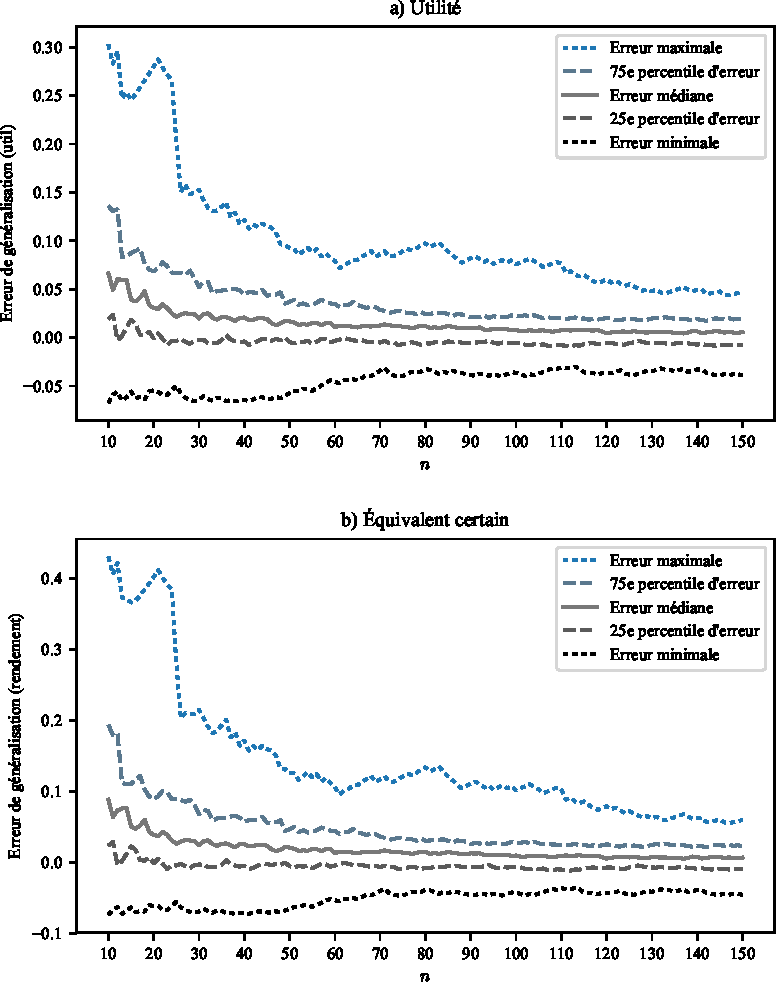
\includegraphics[width=\textwidth]{../experiments/fig/genstats.pdf}
  \caption[Quartiles de l'erreur de généralisation]{Progression des quartiles de l'erreur
    de généralisation en util et en équivalent certain en fonction de la taille $n$ de
    l'échantillonage. Dans environ 75\% des cas, la performance hors échantillon sera
    moindre que celle observée en échantillon. }
  \label{fig_genstats}
\end{figure}


\begin{figure}[h!]
  \centering
  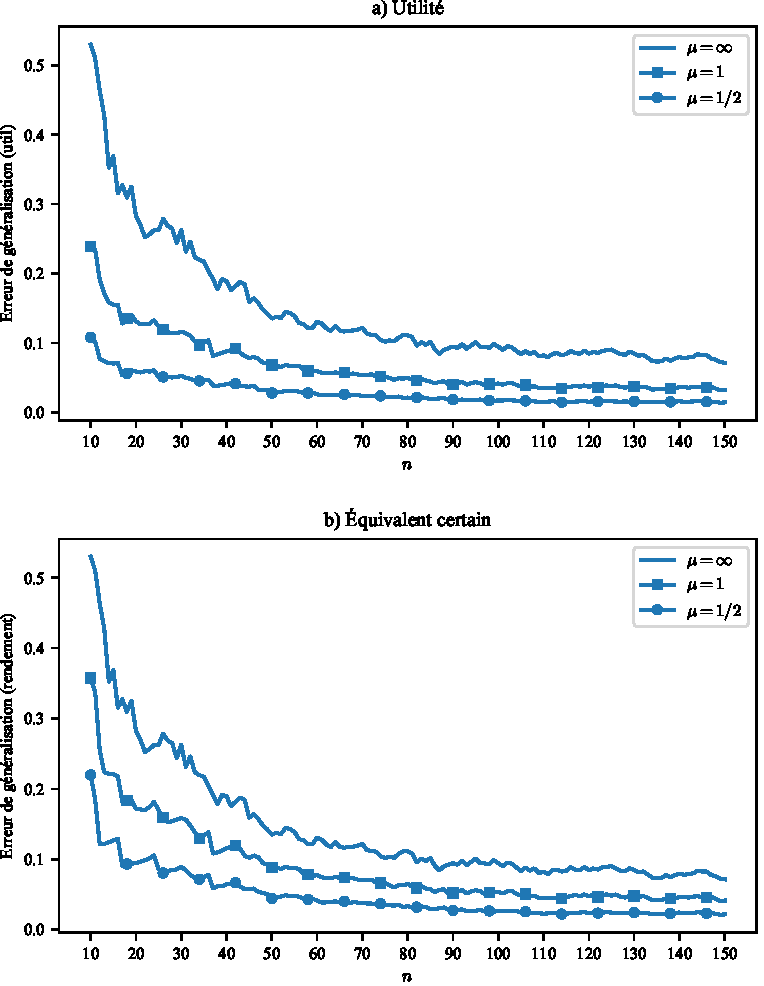
\includegraphics[width=\textwidth]{../experiments/fig/avrisk_gen.pdf}
  \caption[Aversion au risque et erreur de généralisation]{Progression du 95\ieme
    percentile d'erreur de généralisation en fonction de la taille de l'échantillon $n$
    pour trois niveaux d'aversion au risque. Plus l'aversion au risque est faible (avec
    comme cas limite l'attitude neutre au risque $\mu = \infty$), plus l'erreur de généralisation
    est importante, et inversement pour une forte aversion au risque. }
  \label{fig_avrisk_gen}
\end{figure}



\begin{figure}[h!]
  \centering
  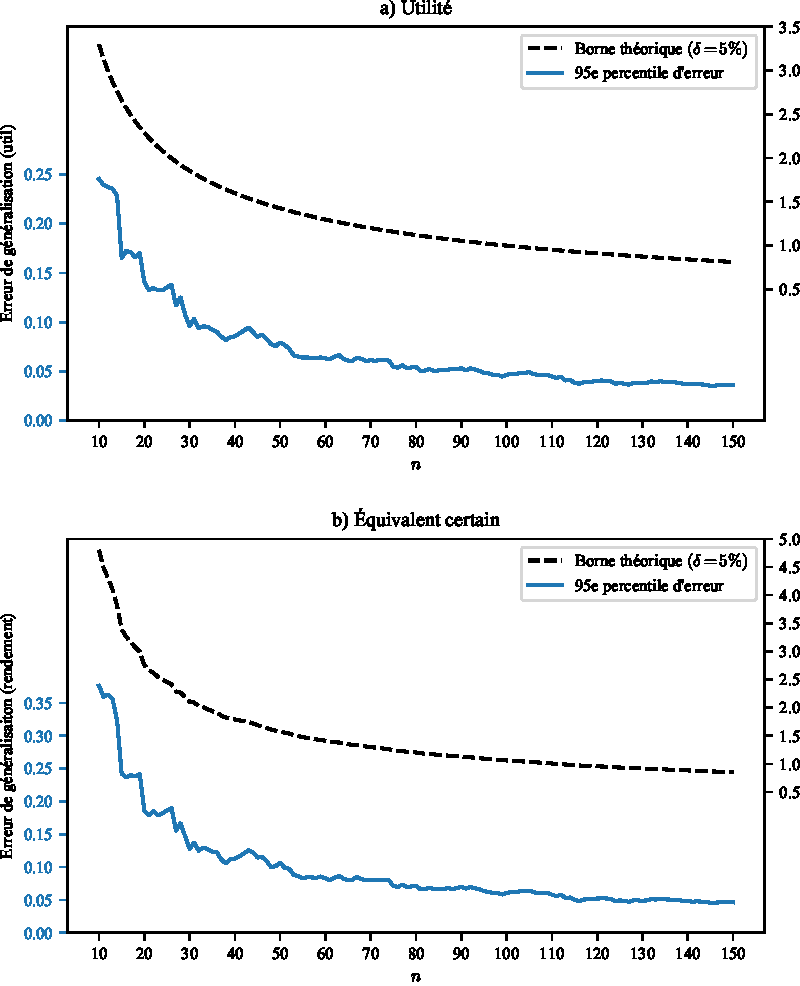
\includegraphics[width=\textwidth]{../experiments/fig/bound_errgen.pdf}
  \caption[Borne théorique sur l'erreur de généralisation]{Progression du 95\ieme
    percentile l'erreur de généralisation et borne théorique (paramètre de confiance
    $\delta = 5\%$) en fonction de la taille d'échantillon $n$, exprimés en util et en
    rendement. Dû à la différence d'ordre, les deux figures font intervenir deux
    ordonnées: celle de gauche quantifie l'erreur empirique alors que celle de droite
    quantifie la borne théorique. Ainsi, la borne théorique est environ 10 fois supérieure
    à l'erreur empirique.}
  \label{fig_bound_errgen}
\end{figure}

\begin{figure}[h!]
  \centering
  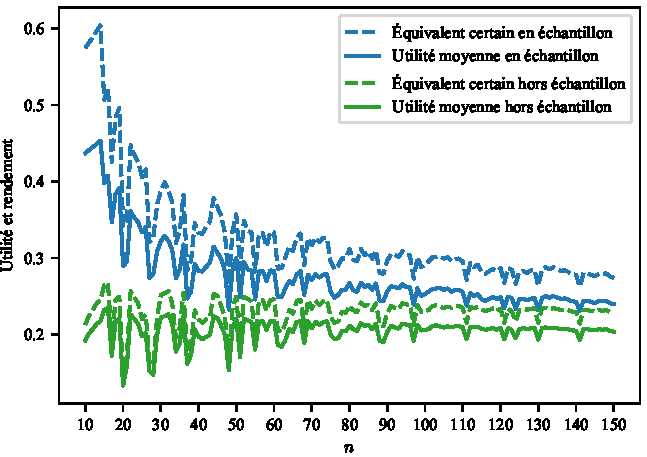
\includegraphics[width=\textwidth]{../experiments/fig/bound_gencomps.pdf}
  \caption[Composantes de l'erreur maximale]{Progression sur la même échelle des
    composantes de performance en échantillon et hors échantillon, exprimées en util et en
    rendement, du 95\ieme percentile d'erreur de généralisation de la Figure
    \ref{fig_bound_errgen} a). Plus une valeur d'utilité est grande, plus l'amplification
    de l'utilité inverse se fera ressentir. L'erreur de généralisation est donc plus
    importante lorsqu'elle est mesurée en unités de rendement qu'en unités d'utils.  }
  \label{fig_bound_gencomps}
\end{figure}

\clearpage


\subsubsection{Erreur de sous optimalité}

Contrairement à l'erreur de généralisation, l'erreur (en util) de sous optimalité
$\EU(\qs) - \EU(\qh)$ (resp.~$\CE(\qs) - \CE(\qh)$ dans le domaine des rendements) ne
bénéficie pas d'une convergence vers zéro du fait de la présence du terme de
régularisation dans l'algorithme $\alg(\S_n)$. En fait, la meilleure garantie offerte par
le théorème \cit, lorsque $n\to\infty$, correspond à $\lambda\|\qs\|^2$ dans le domaine des utils.

Ainsi, la Figure \ref{fig_bound_errso} présente la progression du 95\ieme percentile de
l'erreur empirique de sous optimalité et de la borne théorique $\delta = 5\%$ selon la taille
$n$ de l'échantillon. En particulier, le facteur de régularisation constant
$\lambda = 1/2$ fait en sorte que, exprimés en utils, la borne théorique converge vers
$\lambda\|q^\star\|^2$ (évaluée numériquement à \num{3.16}) alors que le 95\ieme percentile d'erreur
semble converger vers une utilité espérée aux alentours de \num{0.24}.

D'autre part, la borne théorique de sous optimalité du 95\ieme percentile d'erreur
empirique est relâchée d'environ deux ordres de grandeur ($10^{-1}$ pour l'erreur
empirique \textit{vs} $10^{2}$ pour la garantie théorique). En fait, ce qui est
particulièrement déconcertant, c'est que même dans la limite $n\to\infty$, la borne théorique est
supérieure à la plus grande erreur empirique observée (\ie\ lorsque $n=10$)! \todo{En
  fait, il est possible que ce ne soit pas un hasard, mais bien une propriété mathématique
  de l'algorithme.} Cela étant, même si la borne de sous optimalité est particulièrement
relâchée, elle suggère en revanche un ordre de convergence $\bigO(n^{-1/2})$ qui lui
semble être en adéquation avec le 95\ieme percentile de l'erreur de sous optimalité
empirique.

Néanmoins, un investisseur ayant à cœur une faible erreur de sous optimalité devra
nécessairement faire converger son paramètre de régularisation vers zéro à mesure que de
nouvelles observations de la loi de marché sont disponibles. De plus, il a été démontré au
cours de la section précédente qu'on doit avoir $\lambda = \omega(1/\sqrt{n})$, \ie\ une décroissance
moins rapide que $\bigO(1/\sqrt{n})$ pour bénéficier d'une convergence vers une erreur
nulle. En particulier, si $\lambda = \bigO(n^{-k})$, alors la garantie théorique sera composée
de trois termes : $\bigO(n^{k-1}) + \bigO(n^{k-1/2}) + \bigO(n^{-k})$. Dans de telles
conditions, une constante $k=1/4$ semble bien adaptée pour balancer les deux derniers
termes.

Ainsi, la Figure \ref{fig_bound_errso3} présente la progression du 95\ieme percentile
d'erreur de sous optimalité empirique et de sa garantie théorique en fonction de $n$
lorsque $\lambda=(10/n)^{1/4}$. Ainsi défini, lorsque $n=10$, $\lambda$ est identique au facteur de
régularisation employé pour produire la Figure \ref{fig_bound_errso}. On constate
effectivement que l'erreur de sous optimalité est initialement la même pour les deux
figures. Cependant, alors qu'elle paraîssait stagner vers une erreur de 34\% avec une
régularisation constante, la décroissance $\lambda = \bigO(n^{1/4})$ permet ici d'obtenir une
erreur de 26\% lorsque $n=150$. Par contre, il faut être bien conscient que la borne
théorique ne décroît plus qu'à un rythme $\bigO(n^{1/4})$.

\newpage

\begin{figure}[h!]
  \centering
  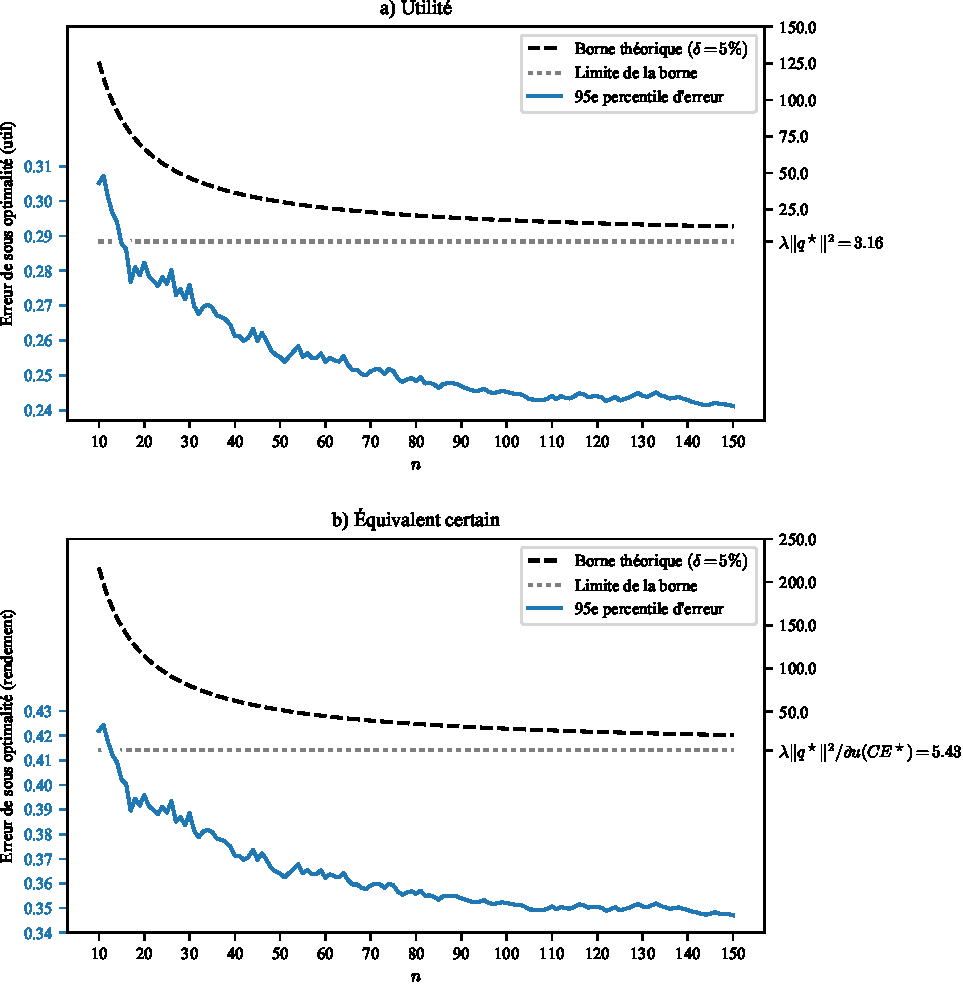
\includegraphics[width=1.3\textwidth]{../experiments/fig/bound_errso.pdf}
  \caption{Progression du 95\ieme percentile l'erreur empirique de sous optimalité et de
    la borne théorique $(\delta = 5\%)$ selon la taille $n$ de l'échantillonage. Le facteur de
    régularisation constant $\lambda = 1/2$ fait en sorte que, exprimés en utils, la borne
    théorique planche à $\lambda\|q^\star\|^2$ (évaluée numériquement à \num{3.16}) alors que le
    95\ieme percentile d'erreur semble plancher aux alentours de \num{0.24}. En plus
    d'être dégagée de près d'un ordre de grandeur de la courbe empirique, même la limite
    de la borne théorique est supérieure aux plus hautes valeurs observées. Cependant,
    l'ordre $\bigO(n^{-1/2})$ théorique se manifeste ici aussi dans le domaine empirique.}
  \label{fig_bound_errso}
\end{figure}

\begin{figure}[h!]
  \centering
  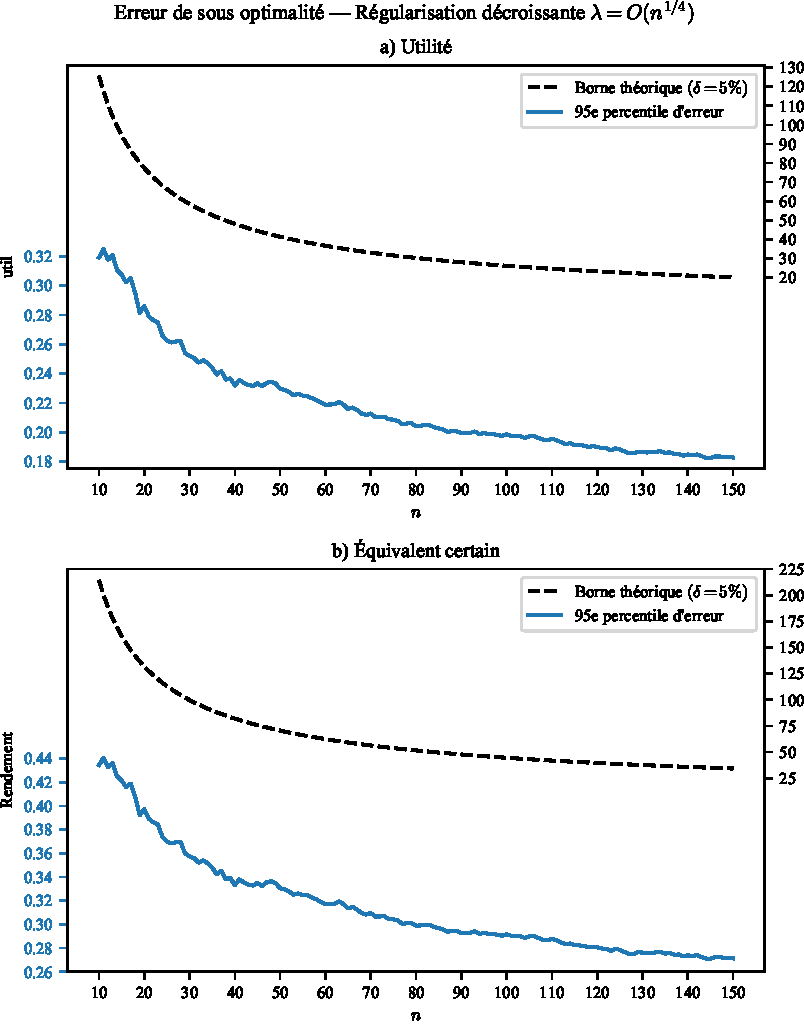
\includegraphics[width=\textwidth]{../experiments/fig/bound_errso3.pdf}
  \caption{Progression du 95\ieme percentile de l'erreur de sous optimalité empirique
    exprimée en util et de la borne théorique $\delta=5\%$ selon la taille $n$ de
    l'échantillonage avec un facteur de régularisation $\lambda = \sqrt{10/n}$. Le panneau a)
    indique la progression de la borne théorique alors que le panneau b) indique sa limite
    de la borne dans le cas $n\to\infty$. Contrairement au cas présenté à la Figure
    \ref{fig_bound_errso}, cette situation offre une garantie théorique d'une erreur nulle
    puisque le facteur de régularisation converge vers 0. Le rythme de convergence n'est
    toutefois que de $\bigO(n^{-1/4})$ alors que l'erreur empirique devrait décroître plus
    rapidement, à un rythme $\bigO(n^{-1/2})$. }
  \label{fig_bound_errso3}
\end{figure}


\clearpage

\subsection{\textit{n} constant, \textit{p} variable}
\label{emp:pvar}

Cette section sera consacrée à l'étude du rapport qu'entretient les erreurs de
généralisation et de sous-optimalité de notre algorithme lorsque sont incorporées à la
prise de décision de nouvelles variables de marché indépendantes des précédantes, tout en
conservant la taille d'échantillonnage constante.

On rappelle donc que les expériences suivantes dévoileront une à une les 50 variables de
marché $X_j$ à partir desquelles le rendement aléatoire $R$ est construit sur une copule
gaussienne. Trois situations différentes seront par ailleurs considérées, chacune d'elles
représentée respectivement par les vecteurs de corrélation
$\Corr(\tilde X,\tilde R) \in \Re^{\bar p}$ (dans le domaine de la copule gaussienne)
suivants:
\begin{gather}
  \rho = \left(\begin{matrix}\sqrt{\frac{1-\epsilon}{\bar p}} & \cdots & \sqrt{\frac{1-\epsilon}{\bar
          p}}\end{matrix}\right)\,;\\
  \rho = \left(\begin{matrix}\sqrt{1-\epsilon} & 0 & \cdots & 0\end{matrix}\right)\,;\\
  \rho = \left(\begin{matrix}0 & \cdots & 0\end{matrix}\right).
\end{gather}

La première situation sera donc celle où chacune des variables de marché a une influence
égale sur le rendement, la seconde celle où seule la première variable vient influencer la
réalisation du rendement et enfin la dernière celle où toutes les variables de marché sont
indépendantes au rendement, \ie\ elle ne forment qu'un ``bruit''. Ces trois situations
seront désignées respectivement par \textit{information dispersée}, \textit{information
  concentrée} et \textit{aucune information}.


\subsubsection{Erreur de généralisation}


La figure \ref{fig_pconst_infogen} présente donc pour ces trois situations comment
progresse leur 95\ieme percentile d'erreur de généralisation (avec $\bar n = 10$
observations du marché) et leur garantie théorique (ici commune aux trois cas) à mesure
que de nouvelles variables de marché sont dévoilées à l'algorithme. Intialement, lorsque
$p=1$ , la courbe \textit{Information concentrée} affiche sans surprise une erreur
beaucoup plus faible que les autres, puisque l'algorithme est déjà en mesure d'inférer la
meilleure politique d'investissement. Au contraire, la courbe \textit{Information
  dispersée} ne détecte qu'un faible lien entre cette variable de marché et $R$. À mesure
que de nouvelles varialbes sont dévoilée, la situation où l'information concentrée
continue de présenter une erreur plus faible aux autres cas, bien que la courbe d'erreur
dans la courbe \textit{Information dispersée} semble finir par la rejoindre. C'est de plus
lorsqu'aucune information n'est présente que le risque d'erreur de généralisation est le
plus grand, puisque toute décision d'investissement non nulle se traduit forcément par une
utilité hors échantillon plus faible qu'en échantillon.

En outre, la garantie sur l'erreur de généralisation, dans le cas d'un apprentissage par
noyau linéaire et d'une taille constante d'échantillonnage, suggère une progression de
l'erreur à un rythme linéaire $\bigO(p)$ (voir Section \ref{b:dim}). Or, les trois courbes
d'erreur empirique semblent indiquer qu'il se pourrait que ce ne soit que le cas que dans
une limite asymptotique. En effet, leur forme est loin d'être linéaire et semble plutôt
posséder une composante racine carrée. Il se pourrait donc que le comportement de l'erreur
de généralisation soit plutôt de $\bigO(p^{1/2}) + \bigO(p)$.

Afin de confirmer cette idée, la figure \ref{fig_pconst_infogen_cf} présente un ajustement
des 25 derniers points des trois courbes d'erreurs empiriques à deux fonctions
polynômiales $f(x) = a_0x + a_1x^{1/2} + b$ et $f(x) = a_0x^{1/2} + b$ par méthode des
moindres carrés. Il faut garder à l'esprit qu'estimer numériquement un ordre polynômial
n'est pas forcément simple, particulièrement lorsqu'on ne dispose que de si peu de points
($\bar p = 50$ dans ce cas-ci). Cela dit, dans les trois cas, l'hypothèse où l'erreur de
généralisation serait de nature $\bigO(p^{1/2}) + \bigO(p)$ semble plus convaincante
puisqu'elle suit de plus proche les vingt cinq premiers points des trois courbes. Cette
conclusion reste cependant spéculative.

\subsubsection{Sous optimalité}

Dans le cas où on ajoute de l'information, la sous optimalité, contrairement à l'erreur de
généralisation, peut référer à deux types d'erreur. Soit on compare la performance hors
échantillon de $\qh$ à celle de la politique optimale qui ne dispose que de
$p \leq \bar p$ variables d'information, soit à la politique optimale qui dispose des
$\bar p$ variables d'information nécessaires pour décrire $M$. Cependant, le développement
théorique qui a été mené au cours de la dernière section ne s'est implicitement préoccupé
que de la première situation.

La Figure \ref{fig_pconst_euinforelative} indique le comportement de l'utilité espérée
optimale $\nEU^\star$ en fonction du nombre de variables de marché connues de
l'algorithme. Naturellement, le cas où toute l'information est disponible dès $p=1$
affiche une utilité espérée optimale constante, alors qu'il s'agit plutôt d'une
progression à peu près linéaire lorsqu'on dévoile progressivement des variables
d'information chacunes faiblement corrélées à $R$, mais indépendantes l'une à
l'autre. Enfin, l'utilité espérée optimale est bien entendu nulle dans le cas où toutes
les variables de marché sont indépendantes à $R$.

La Figure \ref{fig_pconst_infosorelative} elle, indique la progression du 95\ieme
percentile des erreurs de sous optimalité des trois situations et de leur garantie
théorique pour $\delta = 5\%$ à mesure que de nouvelles variables de marché sont dévoilées à
l'algorithme, avec $\bar n = 10$ constant. Initialement, l'erreur de sous optimalité des
courbes \textit{Information dispersée} et \textit{Aucune information} est très faible
alors que la courbe \textit{Information concentrée} dispose déjà de suffisament
d'information pour permettre une erreur élevée. Puis, à mesure que $p$ se rapproche de
$\bar p$, on observe pour la courbe \textit{Information dispersée} une progression qui
correspond environ à la progression de l'utilité espérée optimale. Cela signifie donc que
l'erreur de sous optimalité serait maximisée lorsque l'utilité espérée hors échantillon
est nulle. Les deux autres courbes d'erreur empirique progressent beaucoup plus lentement,
possiblement à un rythme $\bigO(\sqrt{p})$. Dans le cas de la courbe \textit{Information
  concentrée}, puisque sa courbe de référence $\nEU^\star$ est constante, on en conclut
que l'utilité espérée hors échantillon minimale augmente selon $\bigO(\sqrt{p})$. 

De plus, le caractère linéaire annoncé n'est empiriquement pas très clair, sauf dans le
cas particulier où l'information est dispersée. Mais comme c'état le cas pour l'erreur de
généralisation, il n'est pas non plus impossible que l'erreur de sous optimalité ait un
ordre de progression $\bigO(\sqrt{p}) + \bigO(p)$: cela permettrait d'expliquer pourquoi
la courbe \textit{Information dispersée} est linéaire alors que les deux autres affichent
plutôt un caractère de progression racine carrée.
\newpage

\begin{figure}[h!]
  \centering
  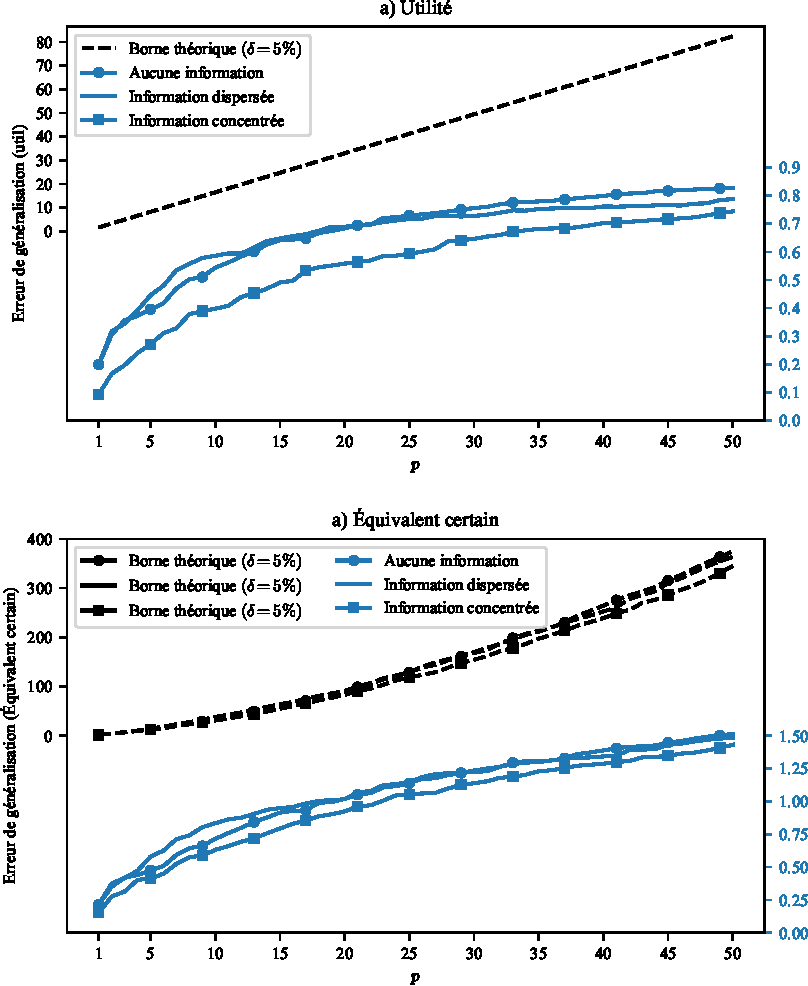
\includegraphics[width=1\textwidth]{../experiments/fig/pconst_infogen2.pdf}
  \caption{Progression du 95\ieme percentile de l'erreur de généralisation exprimée en
    util et en équivalent certain à mesure que de nouvelles variables de marché sont
    dévoilées à l'algorithme, pour une taille d'échantillonnage constante $\bar n =
    10$. Dans le domaine des utils, illustré par le panneau a), la borne théorique est
    commune aux trois situations et progresse linéairement. Lorsque $p=1$, la courbe
    \textit{Information concentrée} affiche sans surprise une erreur initialement plus
    faible que les autres, puisque l'algorithme est déjà en mesure d'inférer la meilleure
    politique d'investissement. Les courbes \textit{Aucune information} et
    \textit{Information dispersée} présentent une erreur similaire lorsque $p$ est faible
    (donc peu de variables connues) mais se distancent l'une de l'autre à mesure que $p$
    converge vers $\bar p$.}
  \label{fig_pconst_infogen}
\end{figure}

\begin{figure}[h!]
  \centering
  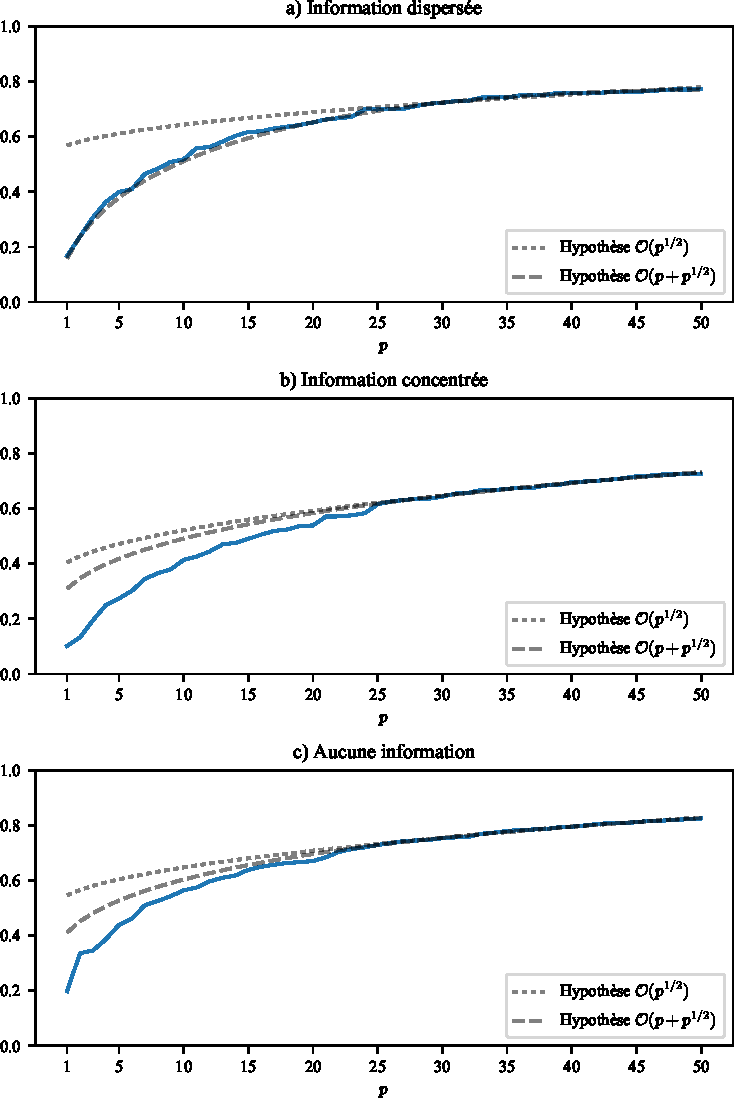
\includegraphics[width=1\textwidth]{../experiments/fig/pconst_infogen_cf.pdf}
  \caption{Ajustement des 25 derniers points des courbes d'erreur présentées à la Figure
    \ref{fig_pconst_infogen} à deux polynômes $f(p) = a_0p + a_1 p^{1/2} + b$ et
    $f(p) = a_0p + b$. Entre les deux, l'hypothèse où l'erreur aurait une progression
    $\bigO(p^{1/2}) + \bigO(p)$ serait ainsi la plus probable.}
  \label{fig_pconst_infogen_cf}
\end{figure}

\clearpage




\begin{figure}[h!]
  \centering
  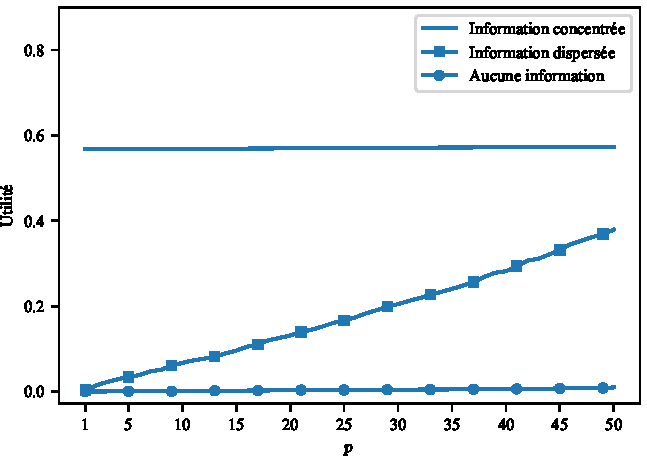
\includegraphics[width=\textwidth]{../experiments/fig/pconst_euinforelative.pdf}
  \caption{Progression de l'utilité espérée optimale $\nEU^\star$ en fonction du nombre de
    variables de marché connues. Naturellement, le cas où toute l'information est
    disponible dès $p=1$ affiche une utilité espérée optimale constante, alors qu'il
    s'agit plutôt d'une progression à peu près linéaire lorsqu'on dévoile progressivement
    des variables d'information chacunes faiblement corrélées à $R$, mais indépendantes
    l'une à l'autre. Enfin, l'utilité espérée optimale est bien entendu nulle dans le cas
    où toutes les variables de marché sont indépendantes à $R$. Les bornes théoriques
    exprimées en util se confondent car elles sont numériquement très rapprochées.}
  \label{fig_pconst_euinforelative}
\end{figure}

\begin{figure}[h!]
  \centering
  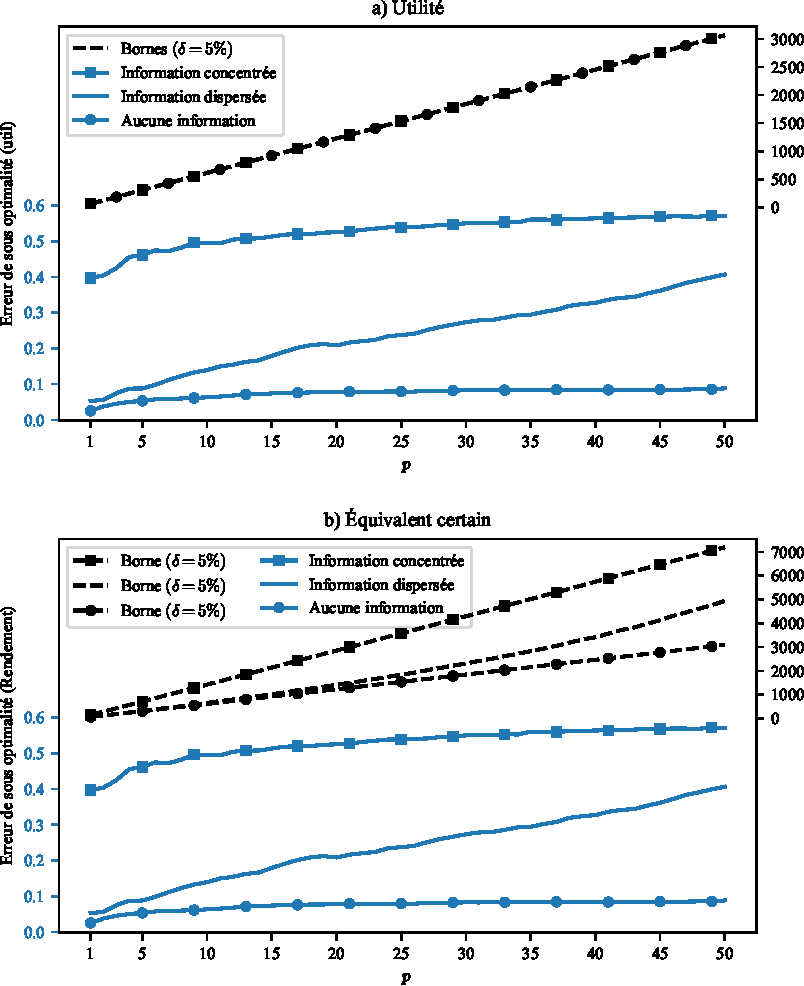
\includegraphics[width=\textwidth]{../experiments/fig/pconst_so.pdf}
  \caption{Progression du 95\ieme percentile des erreurs de sous optimalité et de leur
    garantie théorique à mesure que de nouvelles variables de marché sont dévoilées à
    l'algorithme, avec $\bar n = 10$ constant. Initialement, l'erreur de sous optimalité
    des courbes \textit{Information dispersée} et \textit{Aucune information} est très
    faible alors que la courbe \textit{Information concentrée} dispose déjà de suffisament
    d'information pour permettre une erreur élevée. Puis, à mesure que $p$ se rapproche de
    $\bar p$, on observe pour la courbe \textit{Information dispersée} une progression
    linéaire, alors que l'erreur plafonne dans les deux autres cas. Les garanties en util
    donnent une progression qui elle est linéaire en util. }
  \label{fig_pconst_infosorelative}
\end{figure}


\clearpage

\subsection{$n$ et $p$ variables}
\label{emp:npvar}

Finalement, cette section cherche à illustrer le comportement de l'erreur de
généralisation et de sous optimalité lorsqu'on est en présence de régimes dynamiques entre
$n$ et en $p$, \ie\ lorsque $p=\bigO(n^k)$. Trois régimes seront étudiés : celui où
$p=\bigO(n^{1/2})$, $p=\bigO(n^{3/4})$ et $p=\bigO(n)$. La façon de procéder restera la
même que celle employée aux sections précédentes. Les percentiles d'erreur seront
déterminés à partir d'un échantillon formé de $m=150$ ensembles d'entraînement de taille
$n$, $n$ variant de 9 à 50. Le nombre de variables de marché dévoilées sera ensuite donné
à partir d'une des trois relations suivantes : $p=2n$, $p=3.5n^{3/4}$ et $p=6n^{1/2}$,
selon le régime. Le marché sera constitué de $\bar p = 100$ variables, ce qui correspond à
$p(\bar n)$ dans le régime $p = \bigO(n)$. Ces relations ont été déterminées afin que les
valeurs initiales de $p$ soient identiques et qu'elles conservent le même ordre de
grandeur sur toute l'expérience (voir Figure \ref{fig_np_np}).

\begin{figure}[h]
  \centering
  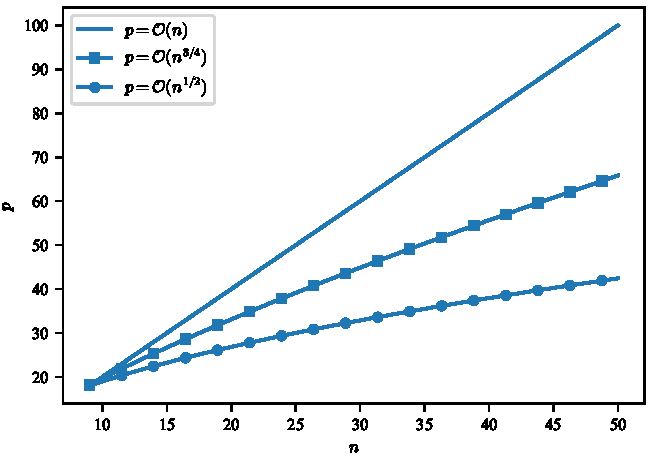
\includegraphics[width=0.7\textwidth]{../experiments/fig/np_np.pdf}
  \caption{En fonction de $n$, trois de cas de figure seront étudiés où le nombre $p$ de
    variables de marché dévoilées à l'algorithme dépend de $n$. Dans les expériences de
    cette section, $n$ variera de $9$ à $50$. La relation entre $p$ et $n$ sera alors
    respectivement donnée par $p = 2n$, $p=3.5n^{3/4}$ et $p=6n^{1/2}$.}
  \label{fig_np_np}
\end{figure}


Les propriétés mathématiques des deux types d'erreur établies à la Section \ref{b:dim}
suggérait un ordre asymptotique $\bigO(p/n^{1/2})$. Les résultats empiriques de la Section
\ref{emp:nvar} (\textit{n} variable, \textit{p} constant) ont d'abord permis de confirmer
l'ordre $\bigO(1/\sqrt{n})$ avec $p$ constant. Puis à la Section \ref{emp:pvar}
(\textit{n} constant, \textit{p} variable), la progression qu'on aurait pu anticiper être
linéaire s'est révélée comporter possiblement une composante racine carrée, \ie\
$\bigO(p) + \bigO(\sqrt{p})$. Ainsi, uniquement à partir de ces observations, on pourrait
conjecturer que l'erreur se comporte en fait comme
$\bigO(p/\sqrt{n}) + \bigO(\sqrt{p/n})$. Du fait de la dominance de $1/\sqrt{n}$ sur
$1/n$, rien n'empêcherait non plus que l'ordre soit $\bigO(p/n) + \bigO(\sqrt{p/n})$.


\subsubsection{Erreur de généralisation}


La Figure \ref{fig_bound_npgenu} présente la progression du 95\ieme percentile de l'erreur
de généralisation et de la garantie théorique ($\delta = 5\%$) des trois régimes de $p$ en
fonction de la taille d'échantillonage $n$. Ce qui frappe surtout, c'est comment les
ordres théoriques n'ont rien à voir avec les ordres empiriques. Soit par exemple le cas où
$p=\bigO(\sqrt{n})$. La courbe de la garantie demeure constante alors qu'en fait c'est
plutôt une décroissance qui est observée. Si on a plutôt une progression $p=\bigO(n)$, il
aurait été raisonnable de penser que l'erreur de généralisation augmenterait, alors que
même dans ce cas, elle continue de décroître!

La Figure \ref{fig_np_np32} présente le 95\ieme percentile de l'erreur de généralisation
suivant un autre régime où $p=0.0016n^{3/2}$. Si l'erreur est alors bien croissante, il
faut être prudent et éviter de généraliser cette observation puisque la valeur de départ
$p = 1$ lorsque $n=9$ n'est pas la même que pour les trois régimes de la Figure
\ref{fig_bound_npgenu} où $p=18$ lorsque $n=9$. Mais de toute façon, les résultats de la
Section \ref{emp:pvar} confirment qu'il existe un point où si $p$ domine suffisament $n$
l'erreur de généralisation devra croître. Il n'est cependant pas clair quel est ce point,
ni comment il dépend de $n$ ou de $p$.


\subsubsection{Erreur de sous optimalité}

La Figure \ref{fig_bound_npgsou} présente quant à elle la progression du 95\ieme
percentile de l'erreur de sous optimalité de la borne de généralisation selon les trois
régimes à l'étude, $p=\bigO(n^{1/2}),p=\bigO(n^{3/4})$ et $p=\bigO(n)$. L'ordre
$\bigO(p/\sqrt{n})$ de la borne théorique semble ici respecté, puisque l'erreur de sous
optimalité demeure constante dans le cas $p=\bigO(\sqrt{n})$, alors qu'elle augmente dans
les deux autres cas. Cependant, les courbes théoriques décroissent, excepté lorsque
$p=\bigO(n)$!

Pour expliquer ce phénomène contre intuitif, il suffit de réaliser que la borne théorique
a en fait une croissance $\bigO(p/\sqrt{n}) + \bigO(\sqrt{p/n}) + \bigO(1)$. Donc si
$p=\bigO(\sqrt{n})$, l'ordre asymptotique de l'erreur sera alors $\bigO(1)$, \ie\ constant
mais le deuxième terme forcera une décroissance $\bigO(\sqrt{n})$ vers cette constante, et
c'est précisément cette décroissance qu'on observe dans la Figure \ref{fig_bound_npgsou}.

De plus, il ne faut pas oublier que la norme de la décision optimale
$\lambda\|q^\star\|^2$ entre aussi dans la composition de la borne théorique, et donc possiblement
dans celle de l'erreur empirique de sous optimalité. Hélas, l'ordre de grandeur de cette
décision optimale est inconnue.

Cette figure illustre en fait assez bien le problème à réduire la progression des erreurs
en ordres asymptotiques. En effet, si l'erreur est polynômiale, alors même si un certain
ordre doit émerger asymptotiquement, lorsque $n$ est fini, il est tout à fait possible que
ce soit un terme d'un autre ordre qui domine la progression.  Avec les paramètres choisis
pour l'expérience de la Figure \ref{fig_bound_npgsou}, si l'ordre de l'erreur de sous
optimalité est effectivement de $\bigO(p/\sqrt{n}) + \bigO(\sqrt{p/n})$, alors il est
clair que seule la première composante joue sur la progression de l'erreur. À la Section
\ref{emp:pvar} où le cas où $n$ étant constant était étudié, il semblait pourtant que
l'erreur progresse en $\bigO(\sqrt{p}) + \bigO(p)$, ce qui laisse donc finalement assez
incertain l'ordre véritable de l'erreur de sous optimalité.


\begin{figure}[h!]
  \centering
  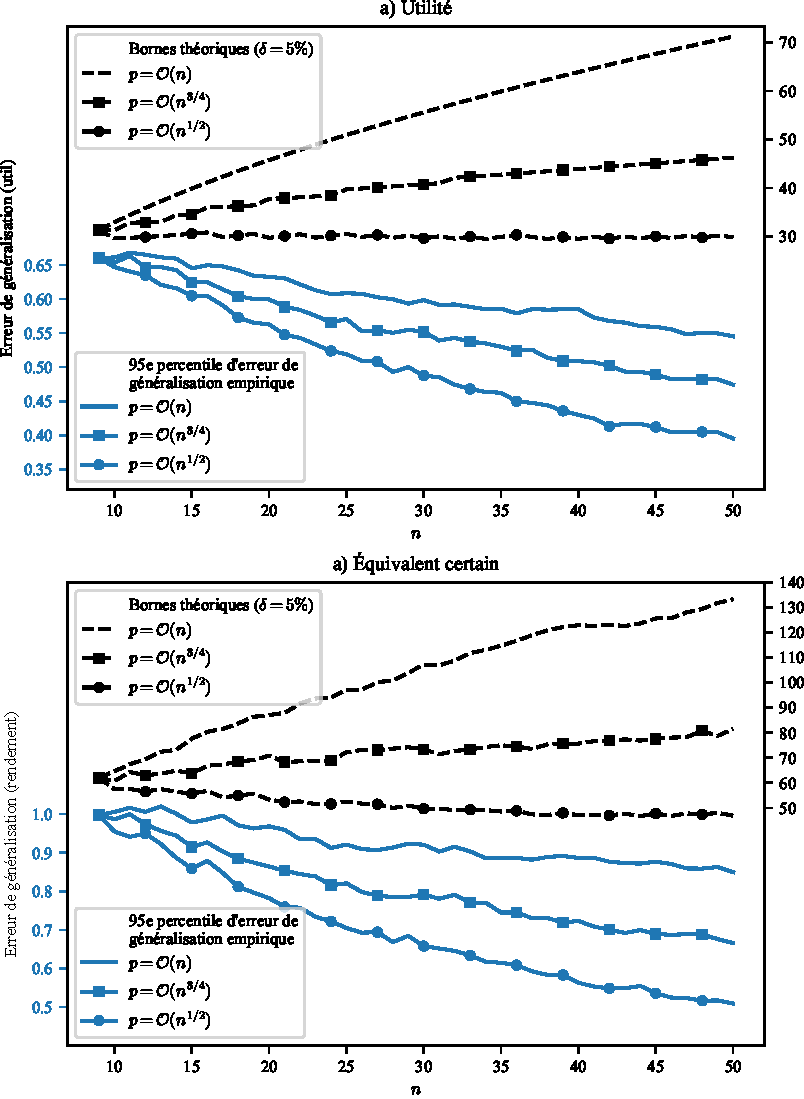
\includegraphics[width=\textwidth]{../experiments/fig/bound_npgenu.pdf}
  \caption{Progression du 95\ieme percentile d'erreur de généralisation et des garanties
    théorique en fonction de $n$, selon le régime de $p$. Une forte disparité entre la
    courbe des garanties théoriques et celle de l'erreur empirique est observée. Les
    courbes théoriques suggérant une progression de l'erreur $\bigO(p/n^{1/2})$, on se
    serait attendu à une amplification de l'erreur dès que $p$ domine $n^{1/2}$, \ie\ si
    $p=\omega(n^{1/2})$. Pourtant, cette figure indique que même si $p$ est de l'ordre de
    $n$, \ie\ $p = \bigO(n)$, l'erreur de généralisation empirique décroit tout de même.  }
  \label{fig_bound_npgenu}
\end{figure}

\begin{figure}[h!]
  \centering
  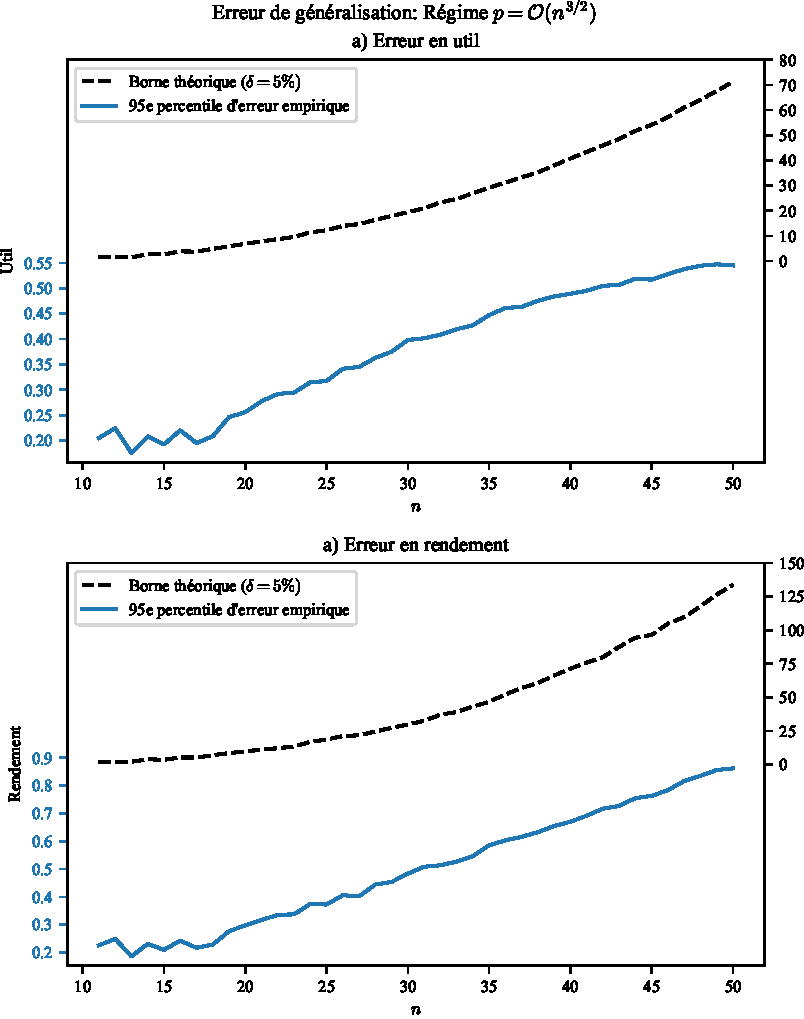
\includegraphics[width=\textwidth]{../experiments/fig/bound_np_np32.pdf}
  \caption{Progression du 95\ieme percentile de l'erreur de généralisation et de sa borne
    théorique $(\delta = 5\%)$ en fonction de la taille de l'échantillonage $n$. La relation
    entre $n$ et $p$ est donnée par la partie entière de $p = 0.0016n^{3/2}$. On observe
    bien une croissance de l'erreur de généralisation, cependant il serait trompeur de
    comparer ce résultat à celui présenté à la Figure \ref{fig_bound_npgenu} puisque le
    nombre $p$ de variables de marché est initialement beaucoup moins élevé dans ce
    cas-ci.}
  \label{fig_np_np32}
\end{figure}

\begin{figure}[p]
  \centering
  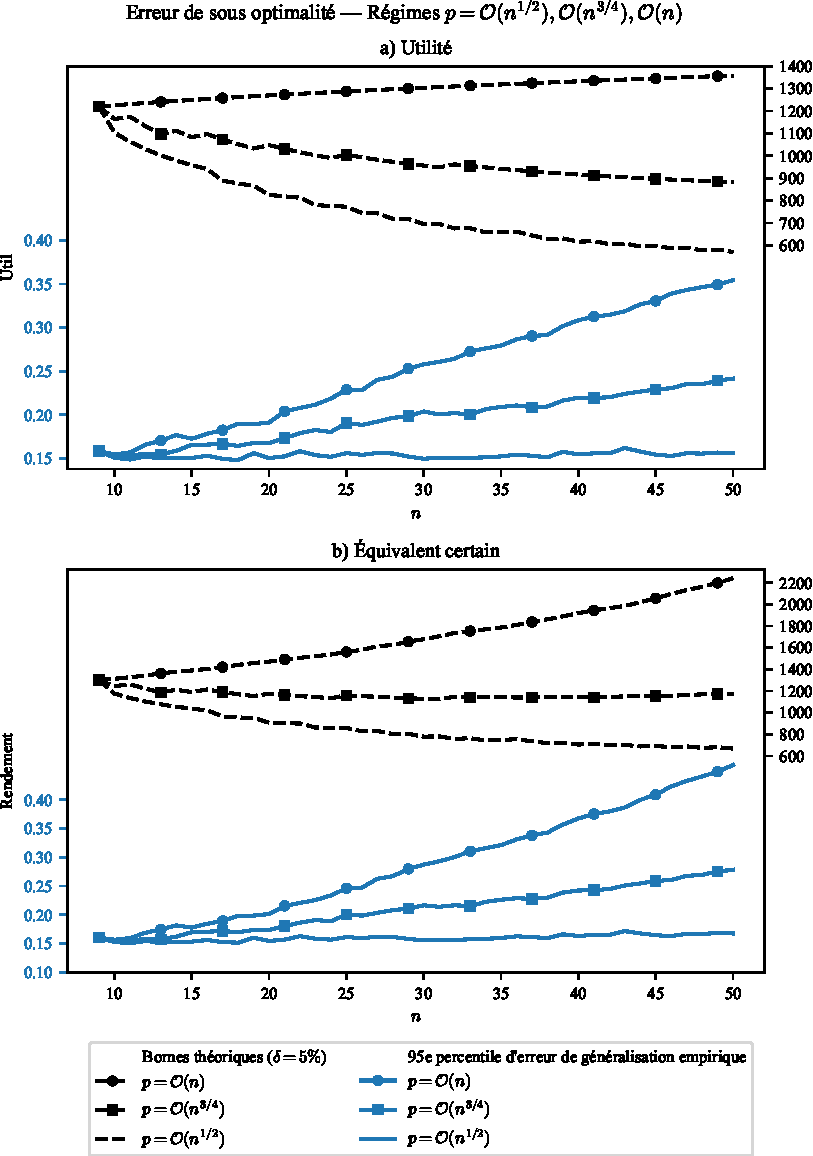
\includegraphics[width=\textwidth]{../experiments/fig/bound_test.pdf}
  \caption[Erreur de sous optimalité -- Régimes $p=\bigO(n^{1/2}),\bigO(n^{3/4}),\bigO(n)$]
  {Progression du 95\ieme percentile de l'erreur de sous optimalité et de sa garantie
    théorique $(\delta=5\%)$ selon les trois régimes à l'étude,
    $p=\bigO(n^{1/2}),p=\bigO(n^{3/4})$ et $p=\bigO(n)$. L'ordre $\bigO(p/\sqrt{n})$ de la
    borne semble ici respecté, puisque l'erreur de sous optimalité demeure constante dans
    le cas $p=\bigO(\sqrt{n})$, alors qu'elle augmente dans les deux autres
    cas. Cependant, les courbes théoriques décroissent, excepté lorsque $p=\bigO(n)$!}
  \label{fig_bound_npgsou}
\end{figure}

\subsection{Conclusion}

Cette section a permis d'illustrer le comportement des erreurs de généralisation et de
sous optimalité dans un cas relativement simple, où l'algorithme de décision ne disposait
que d'un noyau linéaire et où les variables de marché et le rendement étaient toutes
distribuées selon une loi Rademacher, liées les unes autres par une copule gaussienne.

Il a pu être établi assez clairement que pour un nombre constant de variables de marché,
l'erreur décroît bien à un rythme $\bigO(1/\sqrt{n})$, ce qui d'une certaine façon est
sans surprise au su du théorème limite centrale ou de la théorie de la programmation
stochastique \todo{Shapiro}.

Les choses se compliquent sensiblement lorsqu'on fait intervenir un nombre croissant de
variables de marché. Néanmoins, avec $n$ constant, les expériences menées plus haut ont
permis de constater que l'ordre des deux types d'erreur est probablement $\bigO(p)$, bien
que ce régime puisse mettre du temps à apparaître et qu'il serait en fait plus précis de
parler d'un régime $\bigO(p) + \bigO(\sqrt{p})$.

La théorie par contre ne permet pas d'expliquer les courbes d'erreur de généralisation
observées dans des régimes dynamiques où $p=\bigO(n^k)$, où, pour $k\leq1$, celles-ci étaient
toutes décroissantes alors qu'elles auraient dû être croissantes. Ceci dit, l'étude faite
sur l'erreur de sous optimalité viendrait supporter l'idée que sa progression serait bien
de $\bigO(p/\sqrt{n})$. 


\clearpage

% \begin{table}[h]
%   \small
%   \centering
% \begin{tabular}{lrrr}
% \toprule
% $n$ &   $k=1/2$ &  $k=3/4$ &   $k=1$ \\
% \midrule
% 2  &   3 &   4 &   5 \\
% 3  &   4 &   5 &   7 \\
% 4  &   5 &   7 &  10 \\
% 5  &   5 &   8 &  12 \\
% 6  &   6 &   9 &  15 \\
% 7  &   6 &  10 &  17 \\
% 8  &   7 &  11 &  20 \\
% 9  &   7 &  12 &  22 \\
% 10 &   7 &  14 &  25 \\
% 11 &   8 &  15 &  27 \\
% 12 &   8 &  16 &  30 \\
% 13 &   9 &  17 &  32 \\
% 14 &   9 &  18 &  35 \\
% 15 &   9 &  19 &  37 \\
% 16 &  10 &  20 &  40 \\
% 17 &  10 &  20 &  42 \\
% 18 &  10 &  21 &  45 \\
% 19 &  10 &  22 &  47 \\
% 20 &  11 &  23 &  50 \\
% 21 &  11 &  24 &  52 \\
% 22 &  11 &  25 &  55 \\
% 23 &  11 &  26 &  57 \\
% 24 &  12 &  27 &  60 \\
% 25 &  12 &  27 &  62 \\
% 26 &  12 &  28 &  65 \\
% 27 &  12 &  29 &  67 \\
% 28 &  13 &  30 &  70 \\
% 29 &  13 &  31 &  72 \\
% 30 &  13 &  32 &  75 \\
% 31 &  13 &  32 &  77 \\
%   \bottomrule
% \end{tabular}
% \caption{Progression de $p$ par rapport à $n$}
% \label{tbl_np_np}
% \end{table}


% \begin{figure}
%   \centering
%   \caption{Progression de $p$ par rapport à $n$}
%   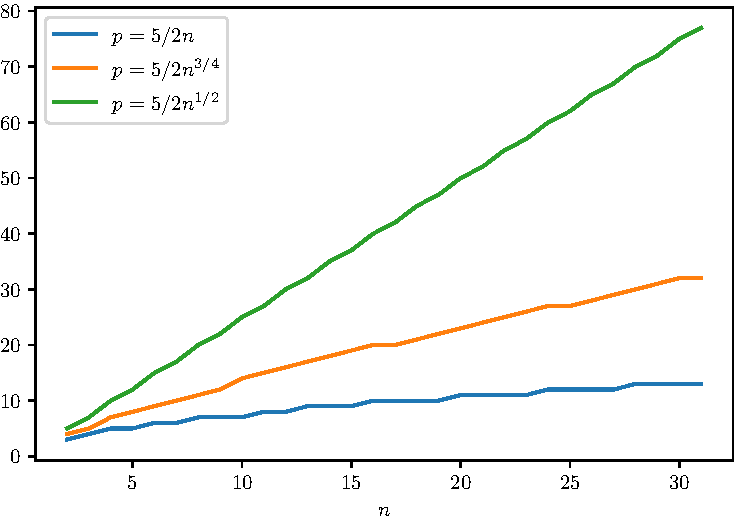
\includegraphics[width=0.8\textwidth]{../experiments/fig/progression1.pdf}
% \end{figure}


% \begin{figure}
%   \centering
%   \begin{subfigure}[b]{\textwidth}
%     \centering
%     \caption{Domaine de l'utilité}
%     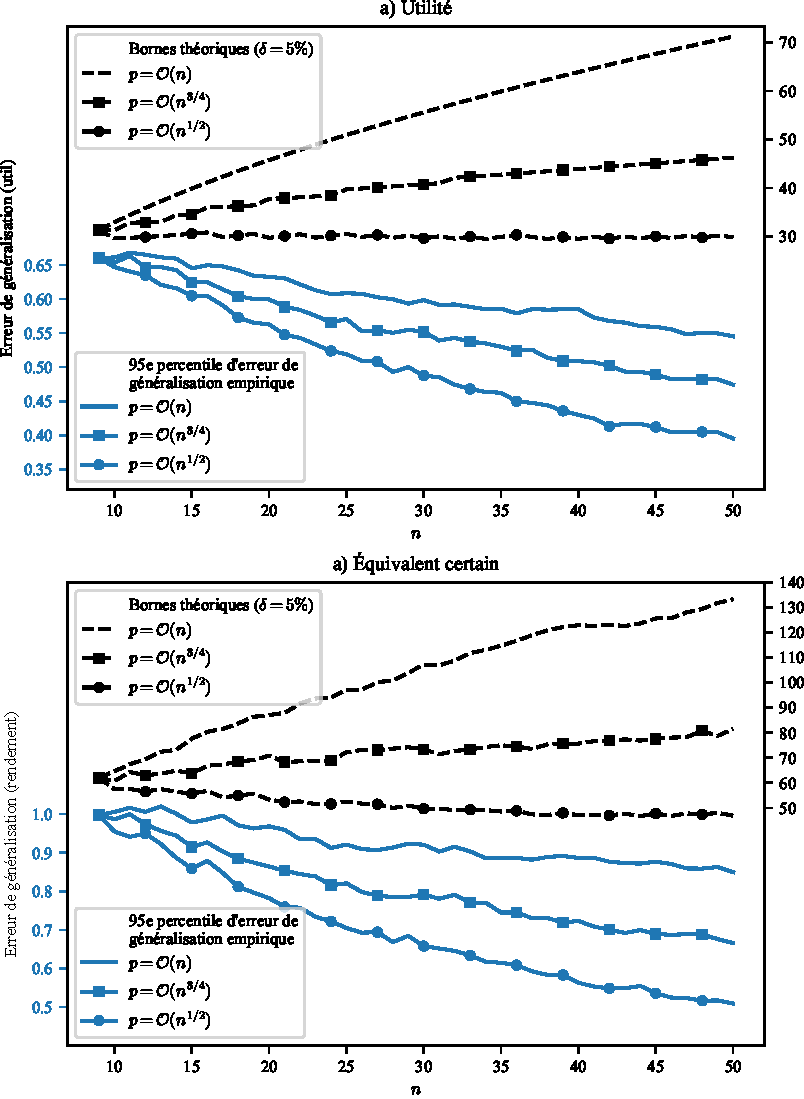
\includegraphics[width=\textwidth]{../experiments/fig/bound_npgenu.pdf}
%   \end{subfigure}
%   \hfill
%   \begin{subfigure}[b]{0.8\textwidth}
%     \caption{Domaine des rendements}
%     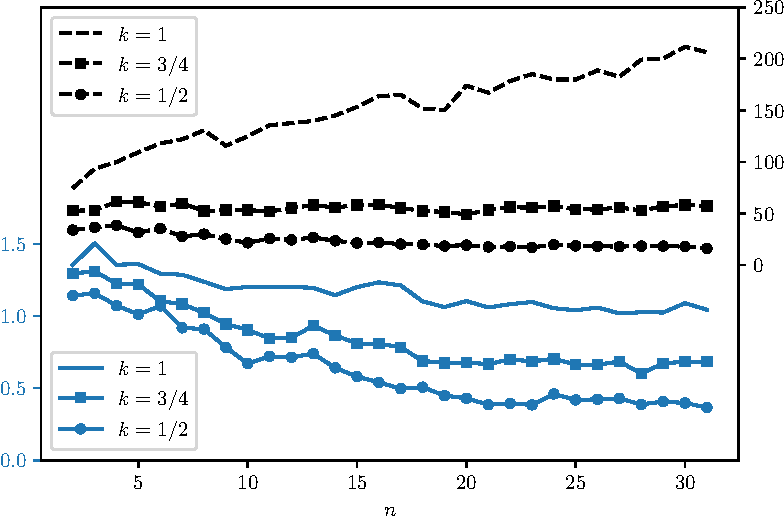
\includegraphics[width=\textwidth]{../experiments/fig/bound_npgence.pdf}
%   \end{subfigure}
%   \caption{Erreur de généralisation -- $n$ et $p$ variables}
%   \label{fig_bound_genu}
% \end{figure}


%%% Local Variables:
%%% mode: latex
%%% TeX-master: "memoire"
%%% End:
